\chapter{Background}
\thispagestyle{document}
\section{Presentation}
	This project gathers three multi-agent systems with forms of intelligence in order to simulate different behaviors.
	
	\subsection{Particles}
	This application simulates a chamber of particles, meaning a finite environment in which particles moves in their own direction and that can collide with other particles or walls of the chamber. The application never stops.
	
	\subsection{Wator}
	This project simulates a game of life in a finite environment with preys (tunas) and predators (sharks). A tuna can only die if eaten by a shark. A shark can only die if it didn't eat after a certain period of time. Tunas and sharks can all reproduce.
	
	The balance of this ecosystem is very delicate: the populations of two species can follow hugely different cycles depending on the given parameters (such as reproduction cycles and the time period in which a shark must eat to avoid starvation) as well as starting positions of each being. We may go from both species being endangered to an abundance of one or both.

When the prey are numerous, predators can reproduce rapidly. But this increase in turn increases the number of prey hunted and the population of the prey decreases. By becoming rarer prey, predators begin to starve and die of starvation, decreasing their population and easing the pressure on hunting prey. The prey (and in time predator) can then go back to rapidly reproducing as the cycle repeats itself.
	\subsection{Hunt}
	
	This project is also a predator-prey system. The prey is guided by the user's gestures on the keyboard and predators use Dijkstra's algorithm to find the shortest path leading to the prey \cite{dijkstra}. Unlike sharks in the wator environment that only eat tunas nearby, the predators have a strategy. Obstacles are also agents but they do not have any intelligence; they just occupy space. The application stops if the prey has been caught by one of the predators.
	
\section{Technical environment}

The project has been developed in the Scala language, using the graphical library ScalaFX to render the views. The project uses SBT (Scala Build Tool) as a build system. All the views in the three applications are canvas, and objects are drawn inside.

The source code of the project can be browsed at this GitHub repository :\\ \url{https://github.com/sallareznov/scalagent}
	
\section{Utilisation}
The project is very easy to use. The three applications can be launched from only one executable archive. To compile the project, use the command \verb+sbt assembly+. This will generate an executable archive named \verb+scalagent.jar+ in the folder \verb+target/scala-2.11/+.

The usage of the program is the following:
\bigskip

\begin{figure}[H]
   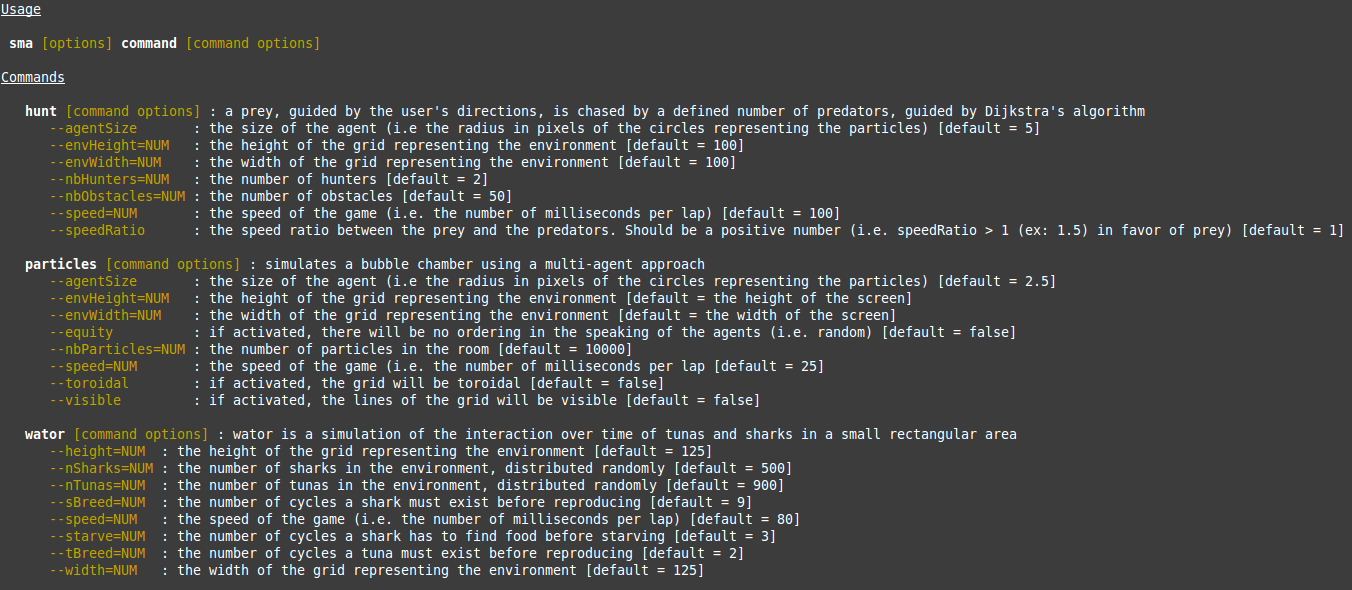
\includegraphics[width=\linewidth]{usage.png}
   \caption{Usage}
\end{figure}

For example, if the user wants to launch the hunt application with default parameters, the command to enter is the following:
\begin{lstlisting}[language=bash]
  $ java -jar scalagent.jar hunt
\end{lstlisting}
\bigskip

If the user wants to use the particles applications with a toroidal grid of 15000 particles, the command to enter is the following:
\begin{lstlisting}[language=bash]
  $ java -jar scalagent.jar particles --nbParticles=15000 --toroidal=true
\end{lstlisting}

PS: For the wator application, the time-dependent number of tunas and sharks and the age pyramid are drawn in real time, during the execution of the application.